\documentclass[11pt]{article}
\usepackage[textwidth=18.0cm, textheight=23.0cm, top=2.0cm]{geometry}
\usepackage{pst-all}
\usepackage{amssymb}
\usepackage{tikz}
\usepackage{underscore}\begin{document}
\pagestyle{empty}


ClassName: \underline{\textbf{Class_08.2bp-7}}
\par
BinSize: \underline{\textbf{100 × 100}}
\par
ReduceSize: \underline{\textbf{100 × 100}}
\par
TypeNum: \underline{\textbf{20}}
\par
Num: \underline{\textbf{20}}
\par
OutS: \underline{\textbf{50000}}
\par
InS: \underline{\textbf{41921}}
\par
Rate: \underline{\textbf{0.838}}
\par
UB: \underline{\textbf{5}}
\par
LB0: \underline{\textbf{5}}
\par
LB: \underline{\textbf{5}}
\par
LBWithCut: \underline{\textbf{5}}
\par
NodeCut: \underline{\textbf{0}}
\par
ExtendedNodeCnt: \underline{\textbf{1}}
\par
GenNodeCnt: \underline{\textbf{1}}
\par
PrimalNode: \underline{\textbf{0}}
\par
ColumnCount: \underline{\textbf{5}}
\par
TotalCutCount: \underline{\textbf{0}}
\par
RootCutCount: \underline{\textbf{0}}
\par
LPSolverCnt: \underline{\textbf{1}}
\par
PricingSolverCnt: \underline{\textbf{0}}
\par
BranchAndBoundNum: \underline{\textbf{1}}
\par
isOpt: \underline{\textbf{true}}
\par
TimeOnInitSolution: \underline{\textbf{600.000 s}}
\par
TimeOnPrimal: \underline{\textbf{0.000 s}}
\par
TimeOnPricing: \underline{\textbf{0.000 s}}
\par
TimeOnRmp: \underline{\textbf{0.062 s}}
\par
TotalTime: \underline{\textbf{600.312 s}}
\par
\newpage


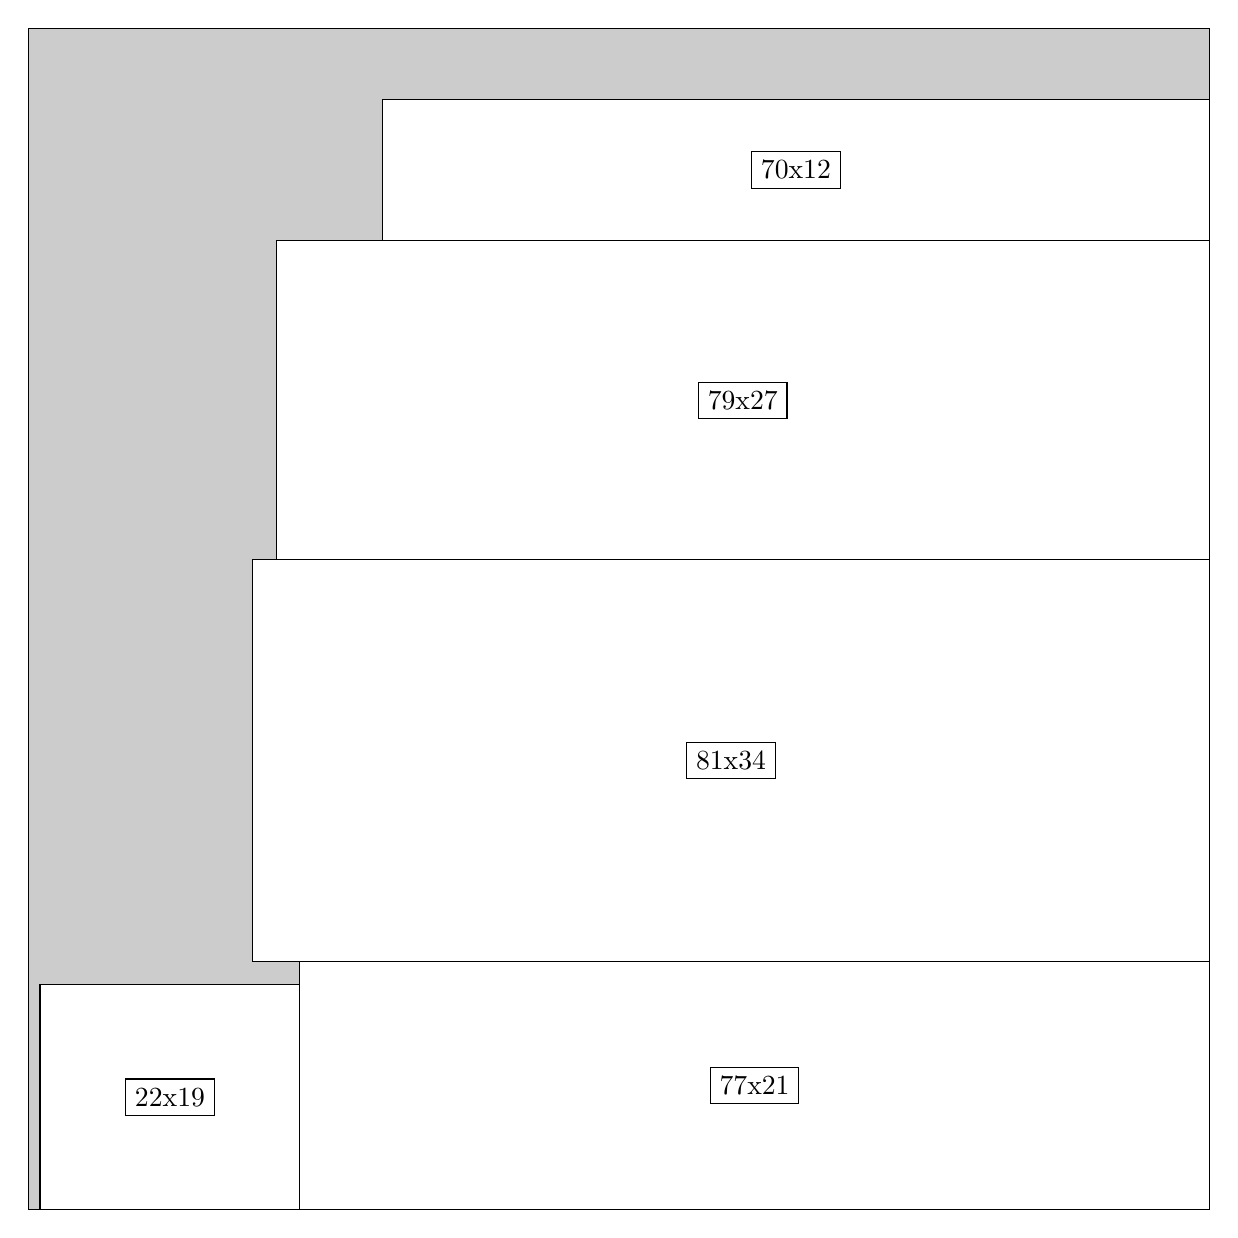
\begin{tikzpicture}[shorten >=1pt,scale=1.0,every node/.style={scale=1.0},->]
\tikzstyle{vertex}=[circle,fill=black!25,minimum size=14pt,inner sep=0pt]
\filldraw[fill=gray!40!white, draw=black] (0,0) rectangle (15.0,15.0);
\foreach \name/\x/\y/\w/\h in {77x21/3.4499999999999997/0.0/11.549999999999999/3.15,22x19/0.15/0.0/3.3/2.85,81x34/2.85/3.15/12.15/5.1,79x27/3.15/8.25/11.85/4.05,70x12/4.5/12.299999999999999/10.5/1.7999999999999998}
\filldraw[fill=white!40!white, draw=black] (\x,\y) rectangle node[draw] (\name) {\name} ++(\w,\h);
\end{tikzpicture}


w =77 , h =21 , x =23 , y =0 , v =1617
\par
w =22 , h =19 , x =1 , y =0 , v =418
\par
w =81 , h =34 , x =19 , y =21 , v =2754
\par
w =79 , h =27 , x =21 , y =55 , v =2133
\par
w =70 , h =12 , x =30 , y =82 , v =840
\par
\newpage


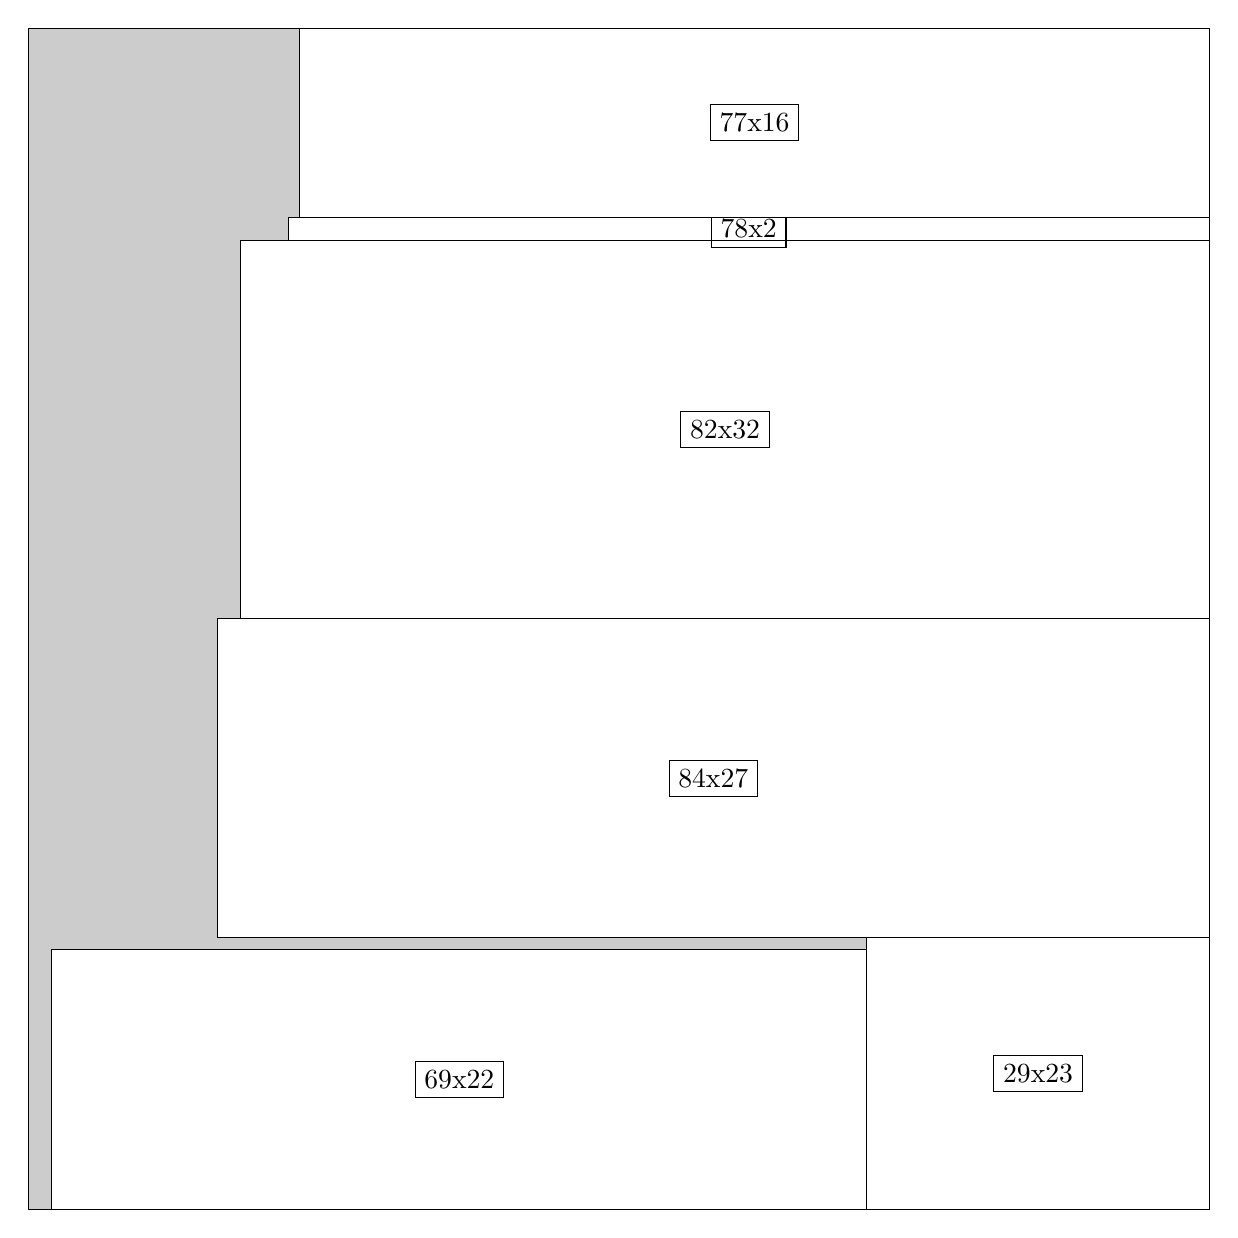
\begin{tikzpicture}[shorten >=1pt,scale=1.0,every node/.style={scale=1.0},->]
\tikzstyle{vertex}=[circle,fill=black!25,minimum size=14pt,inner sep=0pt]
\filldraw[fill=gray!40!white, draw=black] (0,0) rectangle (15.0,15.0);
\foreach \name/\x/\y/\w/\h in {29x23/10.65/0.0/4.35/3.4499999999999997,69x22/0.3/0.0/10.35/3.3,84x27/2.4/3.4499999999999997/12.6/4.05,82x32/2.6999999999999997/7.5/12.299999999999999/4.8,78x2/3.3/12.299999999999999/11.7/0.3,77x16/3.4499999999999997/12.6/11.549999999999999/2.4}
\filldraw[fill=white!40!white, draw=black] (\x,\y) rectangle node[draw] (\name) {\name} ++(\w,\h);
\end{tikzpicture}


w =29 , h =23 , x =71 , y =0 , v =667
\par
w =69 , h =22 , x =2 , y =0 , v =1518
\par
w =84 , h =27 , x =16 , y =23 , v =2268
\par
w =82 , h =32 , x =18 , y =50 , v =2624
\par
w =78 , h =2 , x =22 , y =82 , v =156
\par
w =77 , h =16 , x =23 , y =84 , v =1232
\par
\newpage


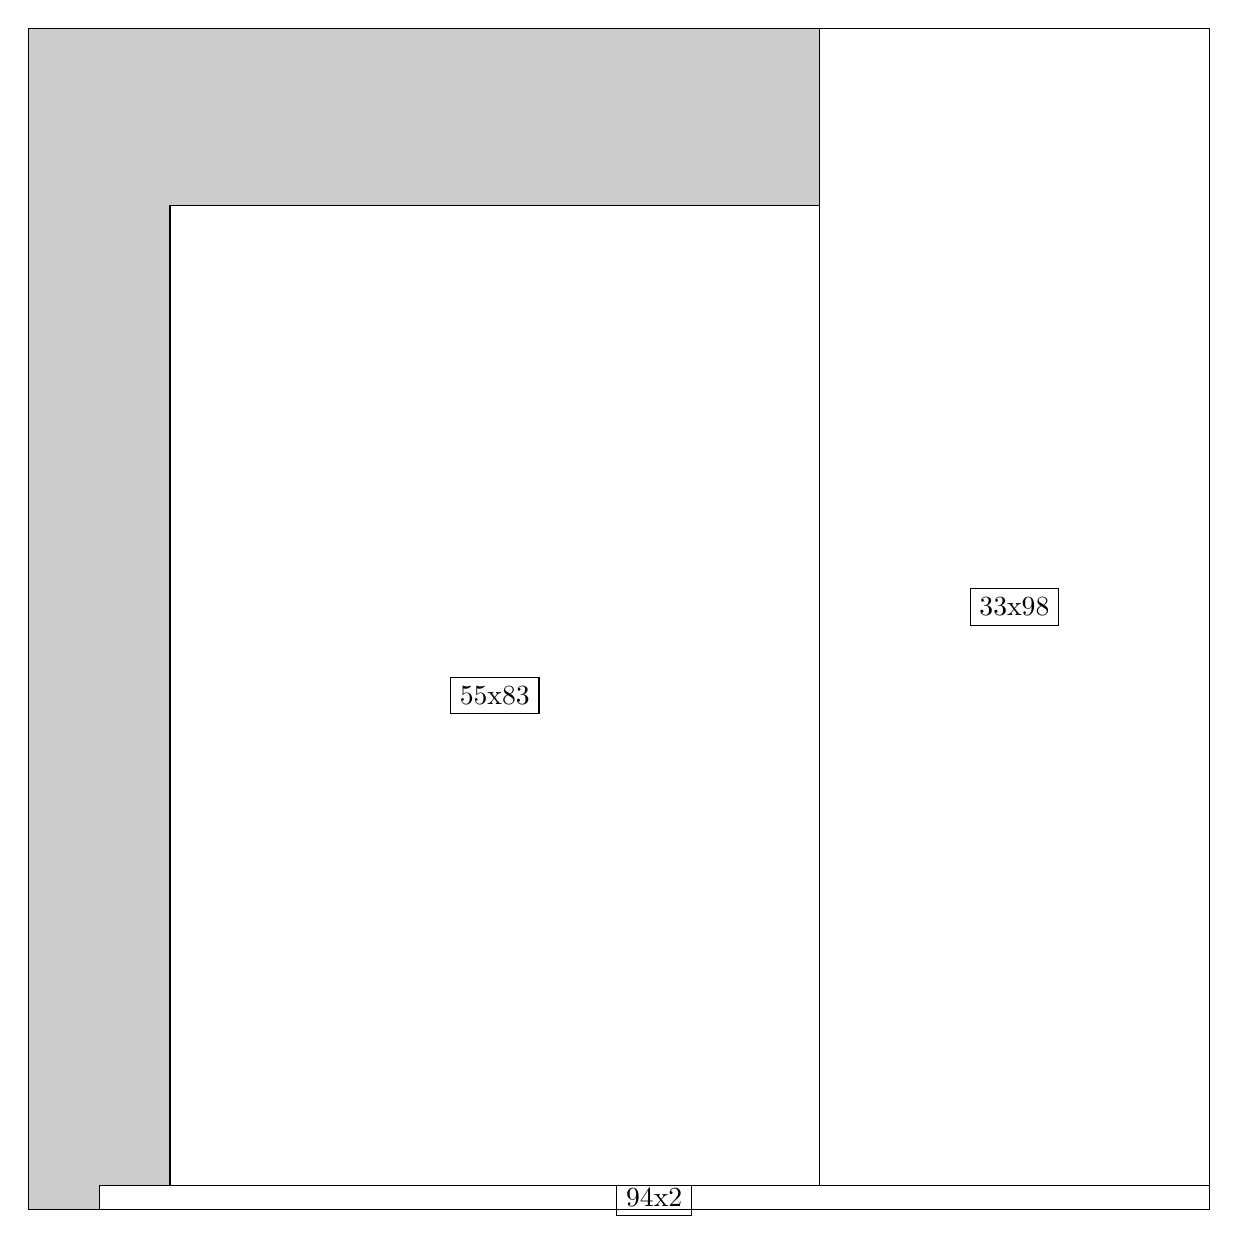
\begin{tikzpicture}[shorten >=1pt,scale=1.0,every node/.style={scale=1.0},->]
\tikzstyle{vertex}=[circle,fill=black!25,minimum size=14pt,inner sep=0pt]
\filldraw[fill=gray!40!white, draw=black] (0,0) rectangle (15.0,15.0);
\foreach \name/\x/\y/\w/\h in {94x2/0.8999999999999999/0.0/14.1/0.3,33x98/10.049999999999999/0.3/4.95/14.7,55x83/1.7999999999999998/0.3/8.25/12.45}
\filldraw[fill=white!40!white, draw=black] (\x,\y) rectangle node[draw] (\name) {\name} ++(\w,\h);
\end{tikzpicture}


w =94 , h =2 , x =6 , y =0 , v =188
\par
w =33 , h =98 , x =67 , y =2 , v =3234
\par
w =55 , h =83 , x =12 , y =2 , v =4565
\par
\newpage


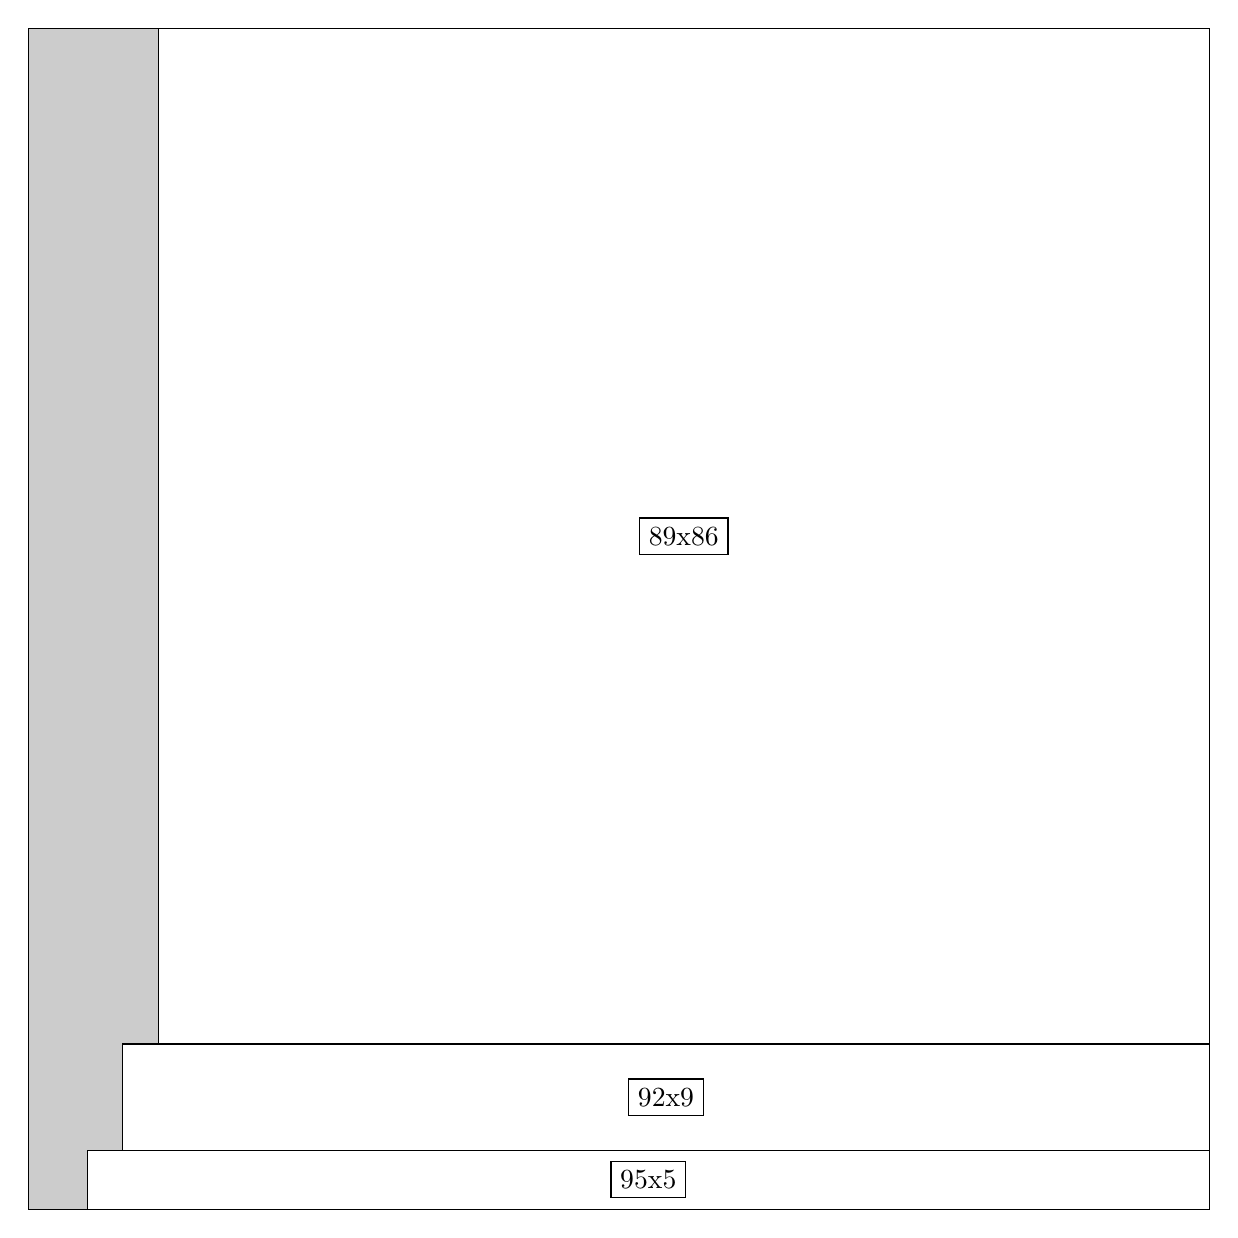
\begin{tikzpicture}[shorten >=1pt,scale=1.0,every node/.style={scale=1.0},->]
\tikzstyle{vertex}=[circle,fill=black!25,minimum size=14pt,inner sep=0pt]
\filldraw[fill=gray!40!white, draw=black] (0,0) rectangle (15.0,15.0);
\foreach \name/\x/\y/\w/\h in {95x5/0.75/0.0/14.25/0.75,92x9/1.2/0.75/13.799999999999999/1.3499999999999999,89x86/1.65/2.1/13.35/12.9}
\filldraw[fill=white!40!white, draw=black] (\x,\y) rectangle node[draw] (\name) {\name} ++(\w,\h);
\end{tikzpicture}


w =95 , h =5 , x =5 , y =0 , v =475
\par
w =92 , h =9 , x =8 , y =5 , v =828
\par
w =89 , h =86 , x =11 , y =14 , v =7654
\par
\newpage


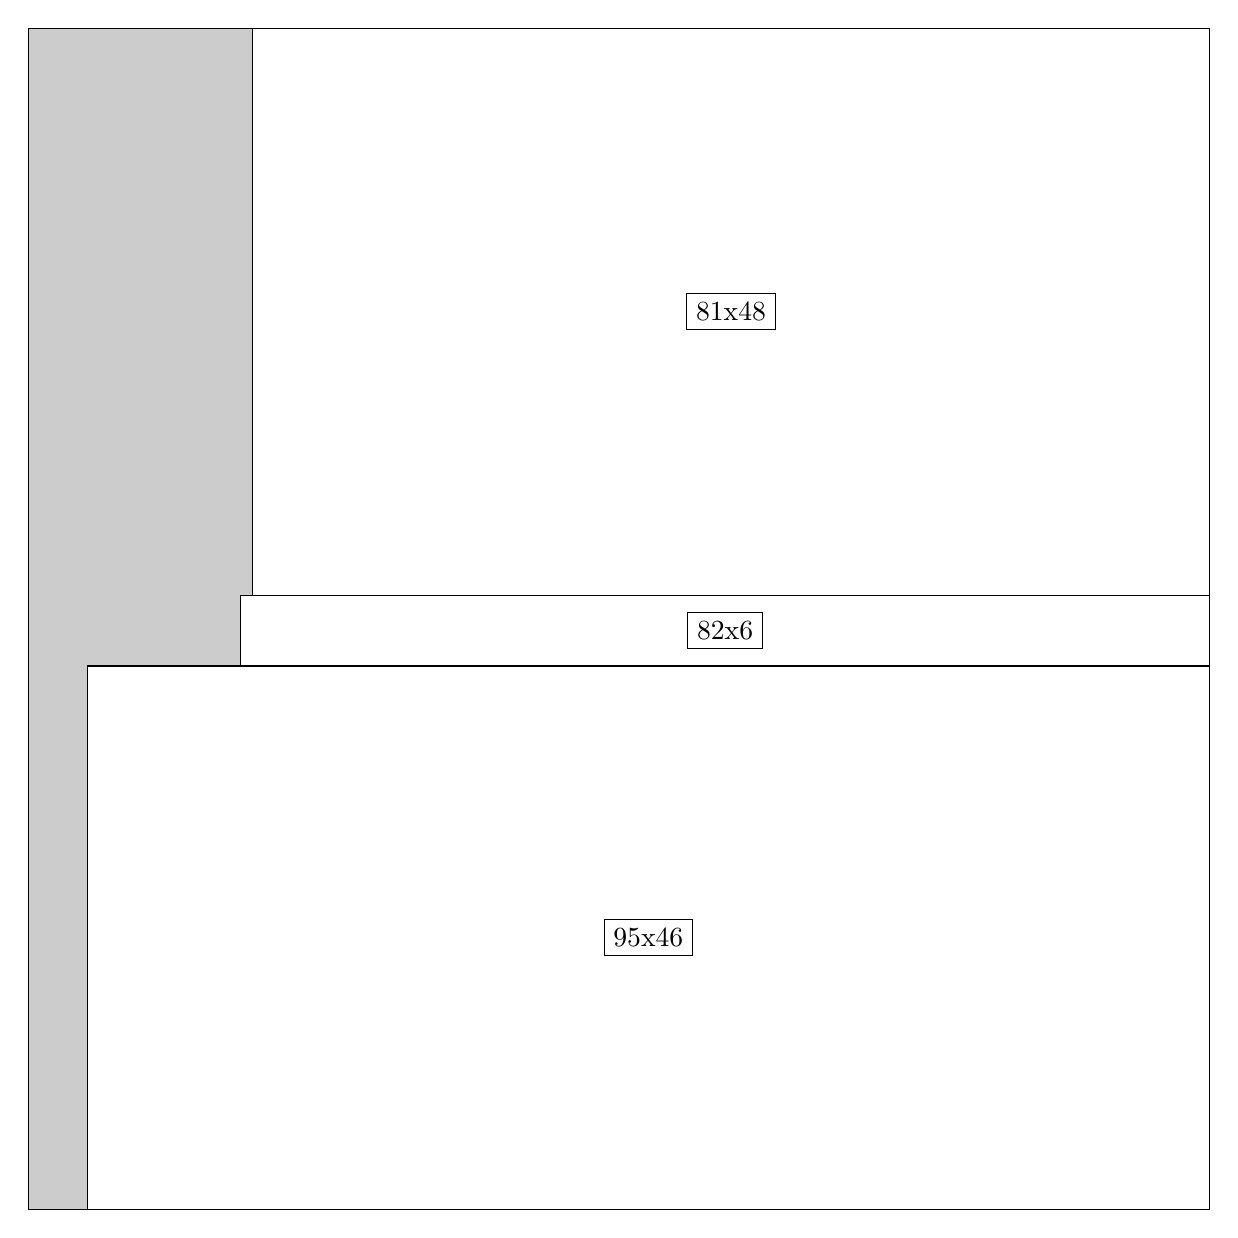
\begin{tikzpicture}[shorten >=1pt,scale=1.0,every node/.style={scale=1.0},->]
\tikzstyle{vertex}=[circle,fill=black!25,minimum size=14pt,inner sep=0pt]
\filldraw[fill=gray!40!white, draw=black] (0,0) rectangle (15.0,15.0);
\foreach \name/\x/\y/\w/\h in {95x46/0.75/0.0/14.25/6.8999999999999995,82x6/2.6999999999999997/6.8999999999999995/12.299999999999999/0.8999999999999999,81x48/2.85/7.8/12.15/7.199999999999999}
\filldraw[fill=white!40!white, draw=black] (\x,\y) rectangle node[draw] (\name) {\name} ++(\w,\h);
\end{tikzpicture}


w =95 , h =46 , x =5 , y =0 , v =4370
\par
w =82 , h =6 , x =18 , y =46 , v =492
\par
w =81 , h =48 , x =19 , y =52 , v =3888
\par
\newpage


\end{document}